This section provides a description of the interaction between TS
system and users (passengers and taxi drivers) and external systems
(GPS system, browser geolocalization and Google Maps). We will put
the accent on the characteristics of each interface.


\subsubsection{User Interfaces }

Since users are not expected to have a technical knowledge, user interface
has to be designed in order to enhance the usability of the software.
In the following, some mockups of the main features available for
the passengers by means of both web and mobile interface will be presented;
they should be considered just a draft.

\begin{figure}[H]
\begin{centering}
\includegraphics[scale=0.4]{\string"specific-requirements/3.1-external-interface-requirements/mockup/png/01 Registrazione 1\string".png}
\par\end{centering}

\protect\caption{Registration form (web interface)}


\end{figure}


\begin{figure}[H]
\centering{}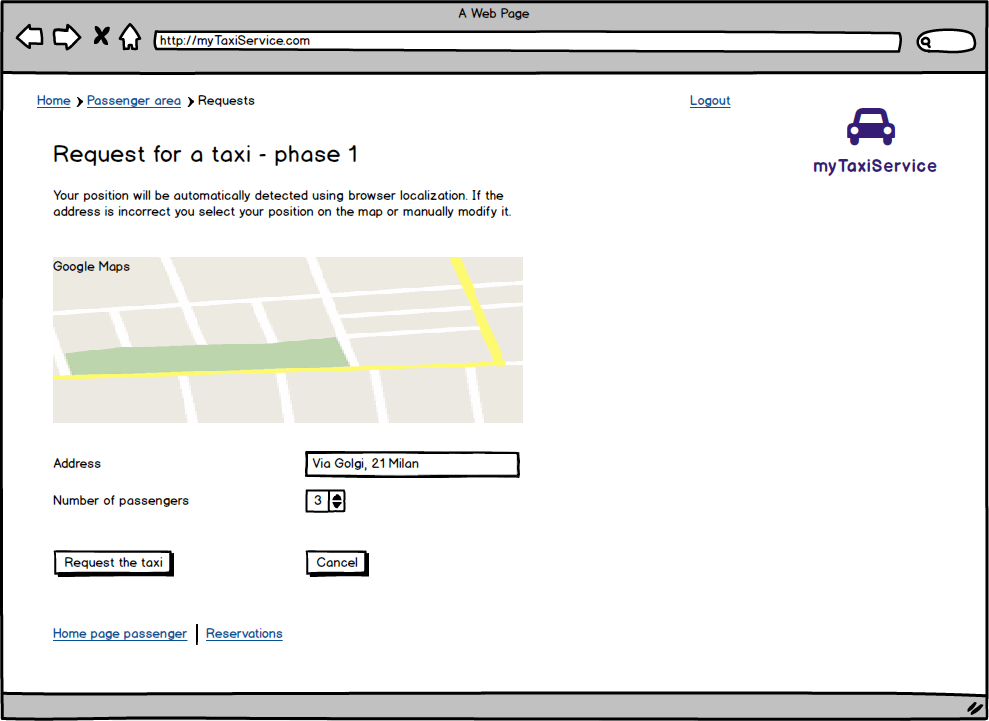
\includegraphics[scale=0.4]{specific-requirements/3.1-external-interface-requirements/mockup/png/request1}\protect\caption{Request for registered passenger 1 (web interface)}
\end{figure}


\begin{figure}[H]
\centering{}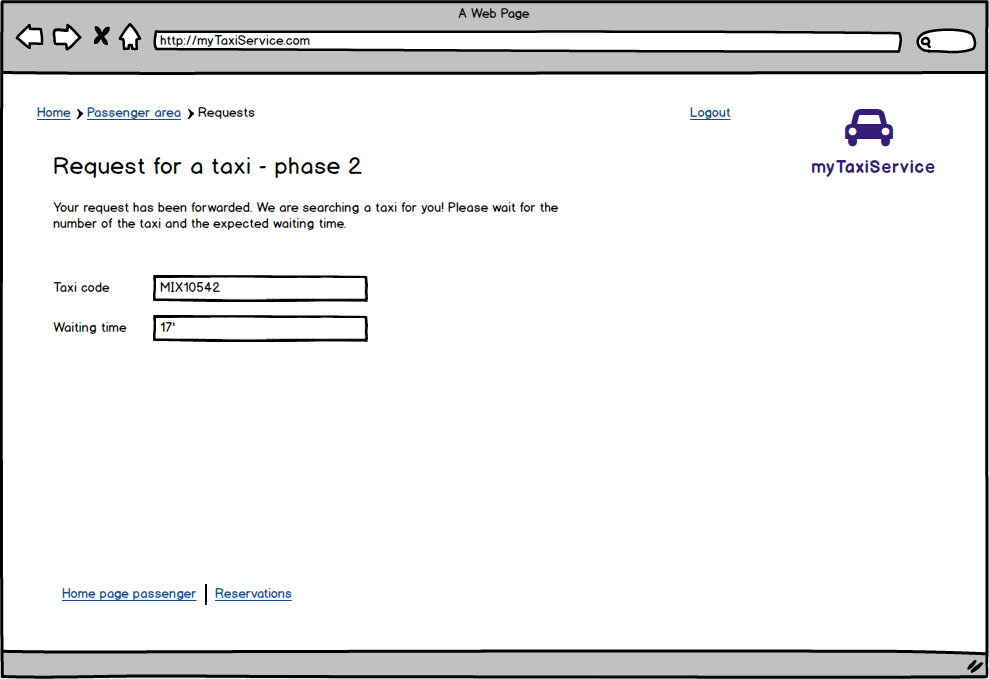
\includegraphics[scale=0.4]{specific-requirements/3.1-external-interface-requirements/mockup/png/request2}\protect\caption{Request for registered passenger 2 (web interface)}
\end{figure}


\begin{figure}[H]
\centering{}\includegraphics[scale=0.4]{\string"specific-requirements/3.1-external-interface-requirements/mockup/png/New Mockup 6\string".png}\includegraphics[scale=0.4]{\string"specific-requirements/3.1-external-interface-requirements/mockup/png/New Mockup 6 copy 3\string".png}\protect\caption{Login (mobile interface) - Modify/Cancel reservation (mobile interface)}
\end{figure}


\begin{figure}[H]
\centering{}\includegraphics[scale=0.4]{\string"specific-requirements/3.1-external-interface-requirements/mockup/png/New Mockup 6 copy\string".png}\includegraphics[scale=0.4]{\string"specific-requirements/3.1-external-interface-requirements/mockup/png/New Mockup 6 copy 2\string".png}\protect\caption{Reservation 1/2 (mobile interface)}
\end{figure}



\subsubsection{Software Interfaces }

TS is interfaced to the following external systems:
\begin{itemize}
\item GPS system of mobile phones for mobile passengers;
\item browser geolocalization for web passengers;
\item Google Maps for the estimation of the waiting time and the specification
of the address when geolocalization or GPS are unavailable.
\end{itemize}
Moreover, TS offers a set of APIs to enable the development of additional
services (e.g., taxi sharing). Those APIs allows developers to have
access the basic functionalists of TS.


\subsubsection{Communication Interfaces }

In order to work properly TS system must have access to the Internet
and all devices involved has to communicate by means of TCP/IP.
